\chapter{Simulation Models and General Approach}\label{chap:approach}
In this chapter the simulation models and their properties will be introduced.
These models will help to describe the physical effects used in the simulation.
The general simulation approach and an overview of ARTS will be presented and discussed in detail.

\section{Receiver and Source Model}\label{sec:receiverAndSource}
\textbf{3D Model}\newline
An acoustic source can be seen as a "speaker" and an acoustic receiver can be seen as a "microphone".
These two have common properties like a location, an orientation which defines their local coordinate system and a field-of-view (FOV) which represents their emission and reception characteristics depending on the outgoing/incoming angle. 
A good receiver FOV example is the human ear.
Turning your ear towards someone who is talking to you will improve the speech reception whereas turning away will decrease it.
We will assume that sources and receivers can be modeled by a single point $(x,y,z)$ in the 3D cartesian coordinate system.
This has been illustrated for the 2D case in \figref{fig:SourceReceiver} in a global coordinate system with $x$-axis and $y$-axis.
\begin{figure}[H]
    \begin{center}
    \subfloat[Receiver Model]{
        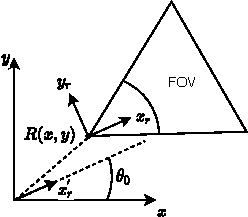
\includegraphics[width=\textwidth/2]{figures/approach/figReceiver.pdf}
    }
    \subfloat[Source Model]{
        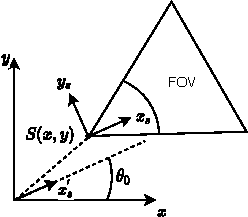
\includegraphics[width=\textwidth/2]{figures/approach/figSource.pdf}
    }
    \end{center}
    \caption[Source and Receiver Properties]{Source and Receiver Properties}
    \label{fig:SourceReceiver}
\end{figure}

Let's define the following conventions for the receiver
\begin{conditions}
    x, y, z         & Location in the global coordinate system \\
    x_r, y_r, z_r   & Local coordinate system with $x_r$-axis, $y_r$-axis and $z_r$-axis \\
    \theta_0        & azimuth angle between global $x$-axis and local $x_r$-axis \\
    \varphi_0       & polar angle between global $z$-axis and local $z_r$-axis
\end{conditions}
and accordingly for the source as well.
Additionally let's define a receiver FOV function 
\begin{equation}
    f_{FOV}(\theta_r, \varphi_r) \rightarrow [0, 1]
\end{equation}
for the reception characteristics and a source FOV function 
\begin{equation}
    g_{FOV}(\theta_s, \varphi_s) \rightarrow [0, 1]
\end{equation}
for the emission characteristics where the respective angles are relative to the local coordinate system.
In \figref{fig:fov} two simple examples are given and how a receiver characteristic could look like.
Evenly distributed (blue rectangle) for a radial receiver without any angle penalty $f(\theta, \varphi)=1$ or linearly decreasing when moving away from the center (red triangle).
The center of the receiver and source is defined by the respective $x_r$- and $x_s$-axis.
\begin{figure}[H]
    \begin{center}
    \subfloat[FOV for $\theta$]{
        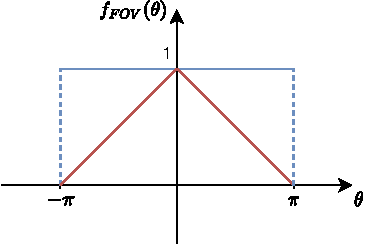
\includegraphics[width=\textwidth/2]{figures/approach/figFovTheta.pdf}
    }
    \subfloat[FOV for $\varphi$]{
        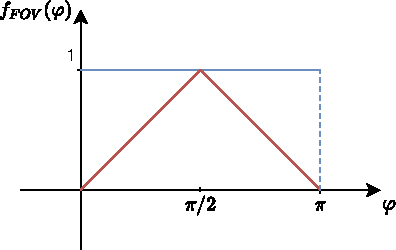
\includegraphics[width=\textwidth/2]{figures/approach/figFovPhi.pdf}
    }
    \end{center}
    \caption[FOV examples]{FOV examples}
    \label{fig:fov}
\end{figure}


\textbf{Receiver and Source Signals}\newline
Even though the geometry of receivers and sources is very similar, the signals are treated differently at the node positions.
A source signal is defined by
\begin{equation}
    s(t) = g_{FOV}(\theta_s, \varphi_s) \cdot x_s(t)
\end{equation}
for $t \in \mathbb{R}_0^+$ and a given direction $(\theta_s, \varphi_s)$ where
\begin{conditions}
    g_{FOV}(\theta_s, \varphi_s)    & Source FOV function \\
    x_s(t)                          & Continuous source signal function, $x_s(t) \rightarrow [-1,1]$ \\
    t                               & time in seconds $[s]$ 
\end{conditions}

The receiver signal on the other hand can be expressed as
\begin{equation}\label{approach:receiver}
    r[n] = f_{FOV}(\theta_r, \varphi_r) \cdot y(n \cdot T_r)
\end{equation}
for $n \in \mathbb{N}$ and a given direction $(\theta_r, \varphi_r)$ where
\begin{conditions}
    f_{FOV}(\theta_r, \varphi_r) & Receiver FOV function \\
    y_r(t) & Continuous receiver signal from direction $(\theta_r, \varphi_r)$, $y_r(t) \rightarrow \mathbb{R}$ \\
    T_r                          & Receiver Sampling Time, $T_r \in \mathbb{R}^+$ \\
    n                            & Sampling index
\end{conditions}

Note how the receiver signal is modeled as a discrete signal and not as a continuous signal.
This is a hint on how the signal is later going to be used.
A real world microphone does record continuously but the signal is later sampled at a given frequency in most systems.

\textbf{Definition}\newline
Given the introduced properties a source $S_i$ is defined by
\begin{itemize}
    \item a global coordinate $(x, y, z)$
    \item rotation $(\theta_0, \varphi_0)$ relative to global coordinate system
    \item output characteristic $g_{FOV}(\theta_s, \varphi_s)$
    \item a source signal $x_s(t)$
\end{itemize}
for $i \in {1,...,M}$ and a receiver $R_j$
\begin{itemize}
    \item a global coordinate $(x, y, z)$
    \item rotation $(\theta_0, \varphi_0)$ relative to global coordinate system
    \item input characteristic $f_{FOV}(\theta_r, \varphi_r)$
    \item sampling frequency $T_r$
\end{itemize}
for $j \in {1,...,N}$.

\section{Obstacle Model}\label{sec:obstacle}
In the model to be presented an "obstacle" is a surface that might reflect or absorb a sound wave.
Other suitable descriptions are "reflector" or "mirror". 
There are stationary obstacles, like walls, windows, doors, tables, TVs and furniture in general and mobile obstacles, like chairs, laptops, bottles and so on.

\textbf{3D Model}\newline
In this approach all types of obstacles are treated the same way and their geometry is defined by (2D-)Polygons with at least three points. If the points form a 2D-polygon they must define a plane $\Phi: ax + by + cz = d$ as well.

\begin{figure}[H]
    \begin{center}
    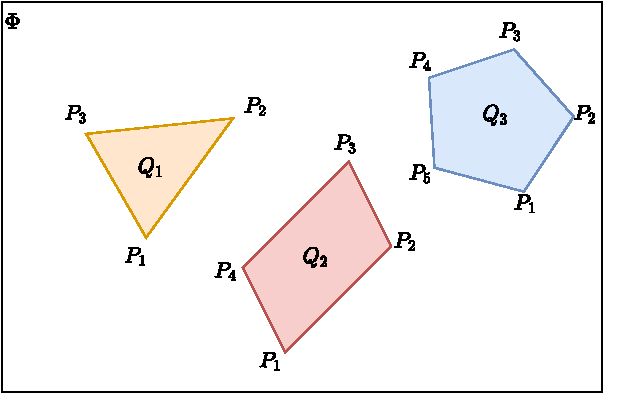
\includegraphics[width=\textwidth]{figures/approach/figObstacles.pdf}
    \end{center}
    \caption[Examples for Obstacles with $N=3,4,5$]{Examples for Obstacles with $N=3,4,5$}
    \label{fig:figObstacles}
\end{figure}


Therefore the geometry of an obstacle $Q_k$ is given by
\begin{itemize}
    \item a set of points $B_k = \{P_1(x,y,z), P_2(x,y,z), ..., P_N(x,y,z)\}$
    \item such that $B_k$ defines a plane $\Phi_k$
\end{itemize}
where $N \geq 3$.

\textbf{Specular Reflection}\newline
When we apply the "geometric acoustic" approach mentioned by Niklas Röber et al in \cite{rober2007ray} sound waves are approximated as particles moving along directional rays.
The reflection of these rays will be modeled the same way as in optics where the reflection angle $\alpha^{'}$ is equal to the incident angle $\alpha$ relative to the surface normal.
\begin{equation}
    \alpha^{'} = \alpha
\end{equation}
Additionally a reflection coefficient $\gamma_k \rightarrow [0,1]$ will be defined, which represents the relation between the outgoing ray intensity level $I_2$ and the incoming ray intensity $I_1$.
\begin{equation}
    \gamma_k = \frac{I_2}{I_1}
\end{equation}
\begin{figure}[H]
    \begin{center}
    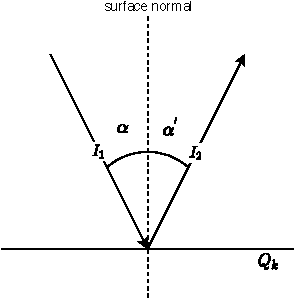
\includegraphics[width=\textwidth/2]{figures/approach/figSpecularReflection.pdf}
    \end{center}
    \caption[Specular reflection]{Specular reflection}
    \label{fig:specularReflection}
\end{figure}

\textbf{Other effects}\newline
As proposed in \cite{rober2007ray} wave phenomena such as "scattering", "diffraction" and the influence of the wavelength are worth mentioning but are usually discarded at higher frequencies.
Since we are looking into ultrasound ($f > 20\text{kHz}$) where the wavelength is much shorter than the dimensions of most obstacles this assumption will be applied for the scope of this thesis.
However these effects are still important for improving the reflection model and for noise generation and they should be introduced at some point.

\textbf{Definition}\newline
Given the discussed properties an obstacle $Q_k$ is defined by
\begin{itemize}
    \item a polygon of set $B_k$ of $N$ coplanar points lying on a plane $\Phi_k$
    \item a reflection coefficient $\gamma_k \rightarrow [0,1]$
\end{itemize}
where $N \geq 3$.

\section{Environment Model}\label{sec:environment}
In \secref{sec:backgroundBasic} we already defined an environment $E$, it is given by the tuple $(\vartheta, \phi, p)$ and a set $Q$ of $K$ obstacles.
The "simplest" environment therefore has no obstacles ($K=0$) and only relies on the temperature $\vartheta$, the relative humidity $\phi$ and atmospheric pressure $p$.
For the environment model these properties are assumed to be static and uniform across space for smaller indoor environments.
Their values will influence certain physical effects such as the speed of sound and mainly "path loss".

\textbf{Speed of sound}\newline
According to Reuben Thomas \cite{wayverb} speed of sound in air can be approximated by

\begin{equation}
    c_{\text{air}} = (331 + 0.6 \frac{\vartheta}{^{\circ}\textrm{C}})\frac{\text{m}}{\text{s}}
\end{equation}

\textbf{Path Loss}\newline
For spherical sound waves (point sources) the intensity in radial direction can be expressed as
\begin{equation}
    I(r) = \frac{P}{4 \cdot \pi \cdot r^2}\label{approach:intensity}
\end{equation}
where
\begin{conditions}
    P & sound power [W] \\
    r & sphere radius [m]
\end{conditions}
The relation $I(r) \propto 1/r^2$ is also referred to as the \textit{inverse-square law}.
Therefore we will approximate the damping of a source signal $s(t)$ by the following loss function
\begin{equation}
    \mathcal{L}(d) = \frac{1}{d+1}\label{approach:loss}
\end{equation}
where
\begin{conditions}
    d & distance travelled [m]
\end{conditions}
Friction and relaxation processes are another source for "path loss" and are described by Russel in \cite{drussell}.
Using Russel's absorption calculator and the values $\vartheta=20^{\circ}\textrm{C}, \phi=0\%, p=101\text{kPa}$ the result is $[6.53 \text{dB}/100\text{m}]$ for 20kHz and $[57.70 \text{dB}/100\text{m}]$ for 60kHz.
Russel shows that "air" can be described as a low-pass filter and that depending on the ultrasonic wave frequency the impact might be huge.
The current model however will for now only rely on the \eqref{approach:loss} as the loss function.

\newpage
\section{Approach Overview}
The general approach is to follow an architecture which is module based.
This will allow us to set clear boundaries for each type of problems while also allowing for optimizations to be made to each individual module independently.
For each module the input is clearly defined and usually results in a single output type which can then be fed to another module.
In the following sections each of these modules will be presented. 
An overview is given in \figref{fig:overview}.

\newpage
\begin{figure}[H]
    \begin{center}
    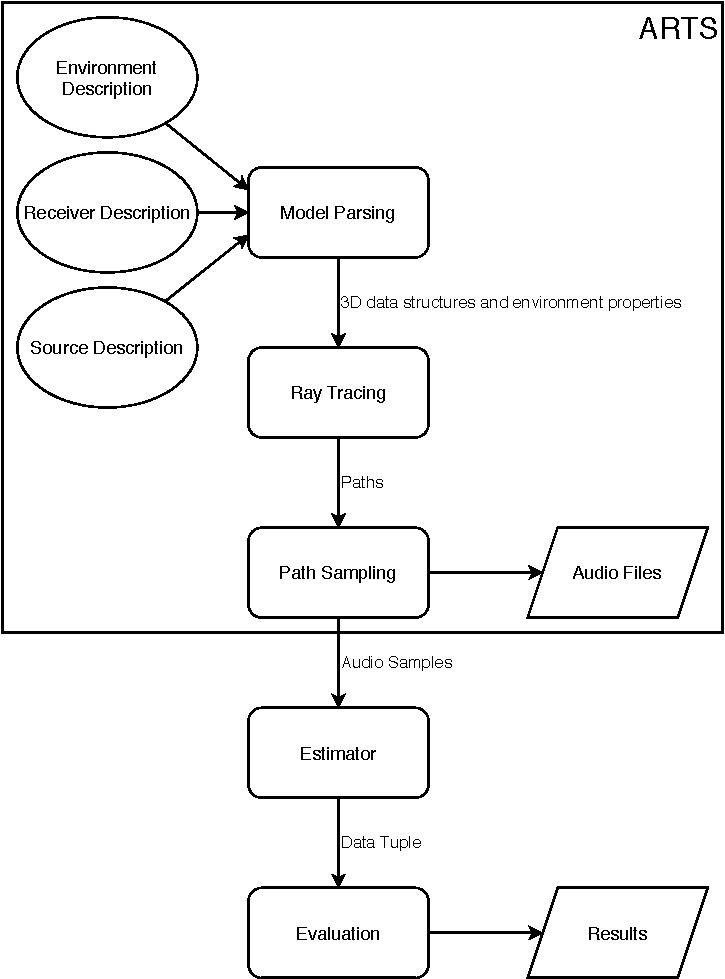
\includegraphics[width=\textwidth]{figures/approach/figOverview.pdf}
    \end{center}
    \caption[Acoustic Ray Tracing Simulator overview]{Acoustic Ray Tracing Simulator overview}
    \label{fig:overview}
\end{figure}

 
\section{Model Parsing}
The Model Parser is the first module of the pursued approach.
It is important that all the properties of a setup $A$ can be loaded in the simulation.
We are dealing mainly with 3D data combined with some physical properties, see \secref{sec:receiverAndSource}, \secref{sec:obstacle} and \secref{sec:environment}.
Therefore a suitable description for these models should be chosen.
The generated 3D data structures and environmental properties will then be used in the following modules.

\begin{figure}[H]
    \begin{center}
    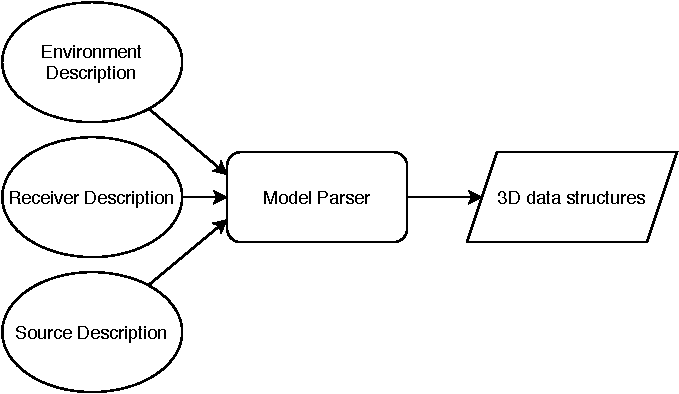
\includegraphics[width=\textwidth]{figures/approach/figModelParser.pdf}
    \end{center}
    \caption[Model Parsing]{Model Parsing}
    \label{fig:modelParser}
\end{figure}


\section{Ray Tracing}
The 3D data structures should represent the sources, receivers and obstacles in a way that simple geometrical operations can be performed, such as "point mirroring", "intersection of rays and obstacles", "distance calculation between points" and so on.
The Ray Tracer should only deal with the geometrical problem of finding paths between sources and receivers.
\begin{figure}[H]
    \begin{center}
    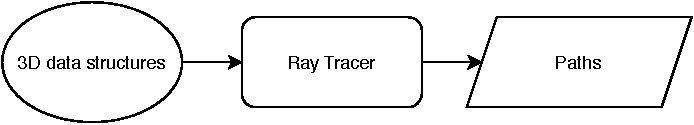
\includegraphics[width=\textwidth]{figures/approach/figRayTracer.pdf}
    \end{center}
    \caption[Ray Tracer Module]{Ray Tracer Module}
    \label{fig:rayTracer}
\end{figure}

The problem to be solved can be stated relatively simple.
For each pair $(S_i, R_j)$, one source $S_i$ and one receiver $R_j$, all possible geometric paths need to be found in an Environment $E$ with $K$ obstacles.

Reflections will be categorized by an Order $L \in \mathbb{N}$. 
They will be referenced as "reflections of order $L$".
The order $L$ tells us how often the ray bounces around until it reaches the receiver $R_j$.
As an example, the special case for $L=0$ is called "direct path" and does not bounce at all.

A Segment $A$ is defined by two locations $A_1(x,y,z)$ and $A_2(x,y,z)$ and a Path $P_{ij}$ is defined by concatenating a sequence of segments, where the starting point is a source $S_i$ and the end point is a source $R_j$. A path can therefore be expressed as

\begin{equation}
    P_{ij} = \{ S_i \rightarrow A_1 \rightarrow A_2 \rightarrow ... \rightarrow A_L \rightarrow R_j\} 
\end{equation}

Let's start with simple examples to figure out the conditions that a source $S_i$ can actually reach the receiver $R_j$.

\textbf{First Condition: No collisions}\newline
A path can only exist if every segment contained does not collide with any obstacle $Q_i$.
Take a look at \figref{fig:collision} for the direct path scenario.
\begin{figure}[H]
    \begin{center}
    \subfloat[Collision-free]{
        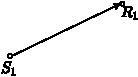
\includegraphics[width=0.5\textwidth]{figures/approach/figNoCollision.pdf}
    }
    \subfloat[Collision detected]{
        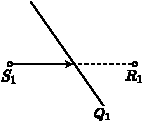
\includegraphics[width=0.5\textwidth]{figures/approach/figCollision.pdf}
    }
    \end{center}
    \caption[Collision cases]{Collision cases}
    \label{fig:collision}
\end{figure}

This condition is true for reflections as well, which consist of $L+1$ Segments.
If the segment starts or ends at a reflection point, the according obstacle should be excluded from this condition.

\textbf{Second Condition: Reflection point exists}\newline
In this example the first order reflection will be considered. 
To ensure that a reflection actually exists two operations need to be performed:
\begin{itemize}
    \item Mirror the receiver point $R_1$ at plane $\Phi_1$ to get the mirroring point $H_1$
    \item Check if segment $(S_1, H_1)$ intersects with the obstacle $Q_1$ in $I_1$
\end{itemize}
\begin{figure}[H]
    \begin{center}
    \subfloat[Reflection of first order]{
        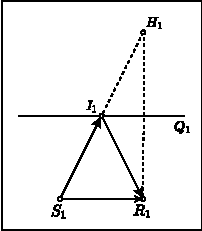
\includegraphics[width=0.5\textwidth]{figures/approach/figReflection.pdf}
    }
    \subfloat[No reflection (intersection point $I_1$ does not exist)]{
        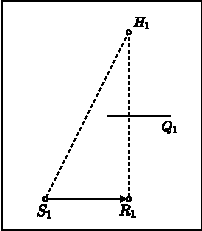
\includegraphics[width=0.5\textwidth]{figures/approach/figNoReflection.pdf}
    }
    \end{center}
    \caption[Reflection cases]{Reflection cases}
    \label{fig:reflection}
\end{figure}

Same as before, this check must hold for higher order reflections as well.

\textbf{Higher order reflections}\newline
For higher order reflections another notation is necessary to distinguish all possible paths and its members.
The previous notation might be enough for first order reflections but a more general description is needed for higher order reflections.
Let $T_l$ be a bounce tuple of length $l \in \{1,...,L\}$ describing a possible obstacle "bounce path".

\begin{itemize}
    \item For first order reflections $L = 1, T_1 = (k_1)$
    \item For second order reflections $L = 2, T_2 = (k_1, k_2)$
    \item For third order reflections $L = 3, T_3 = (k_1, k_2, k_3)$
\end{itemize}
where $k_p \in \{1,...,K\}$ such that $k_{p} \neq k_{p-1}$ for $L > 1$.

A bounce tuple only describes which obstacles $Q_k$ are being visited whereas a regular path describes the sequence of exact locations.
These exact locations for a given tuple $T_l$ are called reflection/intersection point $I_p^{T_l}$ for $p \in \{1,...,L\}$.
In order to get and construct these points the mirrored points $H_p^{T_l}$ for $p \in \{1,...,L\}$ of a receiver $R_j$ are needed.
The existence of these reflection points $I_p^{T_l}$ needs to be confirmed first as we know from the second condition.
An illustration of the notation is given by the example in \figref{fig:higherOrder}.
\begin{figure}[H]
    \begin{center}
    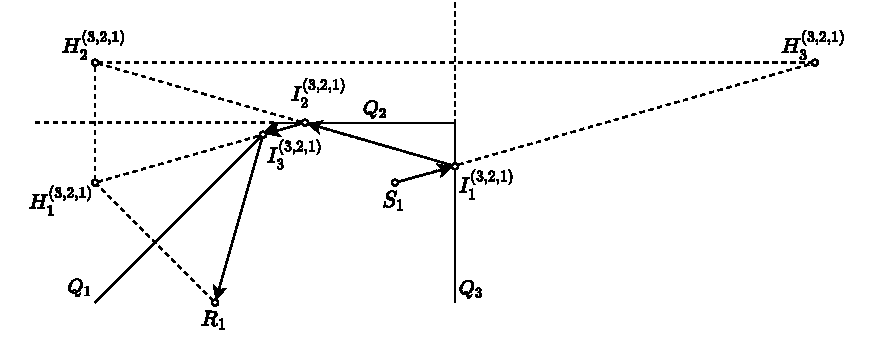
\includegraphics[width=\textwidth]{figures/approach/figHigherOrder.pdf}
    \end{center}
    \caption[$L=3$, Third order example with new notation]{$L=3$, Third order example with new notation}
    \label{fig:higherOrder}
\end{figure}


To summarize the different types of paths:
\begin{itemize}
    \item Direct Path $P_{ij} = \{ S_i \rightarrow R_j \}$
    \item First order path $P_{ij}^{T_1} = \{ S_i \rightarrow I_1^{T_1} \rightarrow R_j \}$
    \item Second order path $P_{ij}^{T_2} = \{ S_i \rightarrow I_1^{T_2} \rightarrow I_2^{T_2}\rightarrow R_j \}$
    \item Third order path $P_{ij}^{T_3} = \{ S_i \rightarrow I_1^{T_3} \rightarrow I_2^{T_3} \rightarrow I_3^{T_3} \rightarrow R_j \}$
\end{itemize}

\textbf{Graphs}\newline
Since the goal is to get all the existing paths for a pair $(S_i, R_j)$ a graph $G_{ij}$ can be described as $G_{ij} = \{P_{ij}\} \cup \{P_{ij}^{T_1}\} \cup \{P_{ij}^{T_2}\} \cup \{P_{ij}^{T_3}\}$ for all existing bounce paths $T_1$, $T_2$, and $T_3$.
An illustration for a "full graph" $G_{ij}$ is given in \figref{fig:graph} for $K=2$ and $L=3$.
\begin{figure}[H]
    \begin{center}
    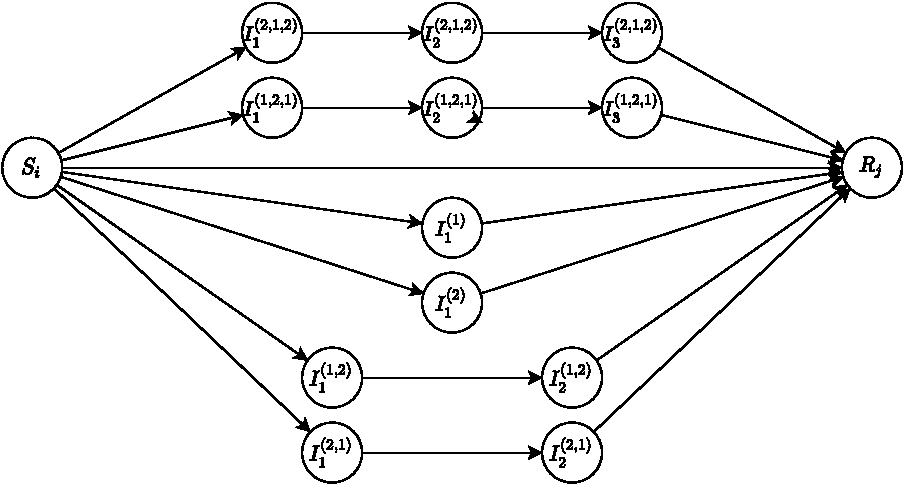
\includegraphics[width=\textwidth]{figures/approach/figGraph.pdf}
    \end{center}
    \caption[Full graph example for $K=2$ and $L=3$]{Full graph example for $K=2$ and $L=3$}
    \label{fig:graph}
\end{figure}


\textbf{Strategy Summary}\newline
For each possible path we need to perform the following actions:
\begin{enumerate}
    \item Mirroring $R_j$ backwards to get mirroring points $H_p^{T_l}$ for $p \in \{1,...,L\}$
    \item Travelling forward to get intersection points $I_p^{T_l}$
    \begin{itemize}
        \item Check if reflection point $I_p^{T_l}$ exists
        \item Check if new segment collides with other obstacles
        \item Add segments to path until $R_j$ is reached
    \end{itemize}
\end{enumerate}

\textbf{Run-time Complexity}\newline
Given that the current strategy is performed on all possible paths the following complexity $C_l$ for a specific order $l > 0, l \in \{1,...,L\}$ can be expected:
\begin{equation}
    C_l = M \cdot N \cdot K \cdot (K-1)^{l-1}
\end{equation}
where
\begin{conditions}
    M & The number of sources $S_i$ \\
    N & The number of receivers $R_j$ \\
    K & The number of obstacles $Q_k$
\end{conditions}

The total number of paths and the total complexity $C_L$ for all full graphs $G_{ij}$ can be expressed as
\begin{equation}\label{eq:complex}
    C_L = M \cdot N + \sum_{l=1}^{L}{C_l} =  M \cdot N \cdot ( 1 + K \cdot \sum_{l=1}^{L}{(K-1)^{l-1}})
\end{equation}

This sets an upper bound for the complexity of the current strategy.
A lot of paths will probably fail to satisfy one of the two checks and therefore terminate earlier.
The first step however is performed for every possible path, therefore run-times of order $C_L$ are expected.

\section{Path Sampling}
The "Ray Tracer" provides a set of paths in form of a Graph $G_{ij}$.
Each path might contribute to the final received signal depending on the properties of a path $P$ in $G_{ij}$ and the environmental properties introduced in the previous chapters.
The "Path Sampler" takes all these modeled effects and creates a set of samples for each $(S_i, R_j)$ pair.

\begin{figure}[H]
    \begin{center}
    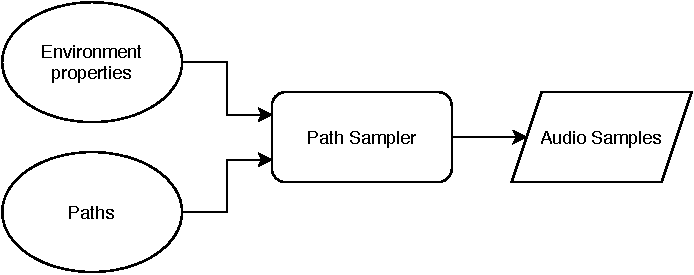
\includegraphics[width=\textwidth]{figures/approach/figPathSampler.pdf}
    \end{center}
    \caption[Path Sampler Module]{Path Sampler Module}
    \label{fig:pathSampler}
\end{figure}

In \eqref{approach:receiver} a first sneak peek was given on how an incoming signal $r[n]$ will be sampled.
A lot of different models have been introduced since then and they will now be condensed into a single equation for the total received signal $r_{ij}[n]$:
\begin{equation}\label{eq:receiver}
    r_{ij}[n] = \sum_{P \in G_{ij}} f_{FOV}(\theta_{r,P}, \varphi_{r,P}) \cdot \mathcal{L}(d_P) \cdot \prod_{\gamma_k \in P}{\gamma_k} \cdot g_{FOV}(\theta_{s,P}, \varphi_{s,P}) \cdot x_s(n \cdot T_r - \frac{d_P}{c_{\text{air}}})
\end{equation}
where
\begin{conditions}
    P & Path in Graph $G_{ij}$ \\
    d_P & Total Path length of $P$ in [m] \\
    f_{FOV}(\theta_{r,P}, \varphi_{r,P}) & Receiver $R_j$ FOV factor for incoming direction of path $P$ \\
    \mathcal{L}(d_P) & Distance $d_P$ loss factor \\
    \prod_{\gamma_k \in P}{\gamma_k} & Combined Reflection factor for all obstacles $Q_k$ in $P$ \\
    g_{FOV}(\theta_{s,P}, \varphi_{s,P}) & Source $S_i$ FOV factor for outgoing direction of path $P$ \\
    x_s(t) & Source signal of $S_i$ \\
    n  & Sampling index \\
    T_r & Receiver $R_j$ sampling time in [s] \\
    c_{\text{air}} & Speed of sound in [m/s]
\end{conditions}

\section{Estimation and Evaluation}
An estimator represents a system that is trying to solve a certain problem.
Indoor localization estimators will most likely try to estimate locations $(x,y,z)$ in the room like in \cite{bordoy2019exploiting}, angle of arrivals (AOA) $(\theta, \varphi)$, time difference of arrival (TDOA) $(t_1, t_2,...)$ and so on.

Indoor mapping applications will try to estimate the room geometry.
This can be expressed as a tuple of normal vectors $(\vec{n_1},\vec{n_2},...)$ for distances to walls and obstacles similar to \cite{ribeiro2011geometrically} or in the best case 3D data structures of the environment.

Another example could be that the simulator should be improved.
Therefore the estimation process can be skipped completely, acting as a pass-through.
This could be very useful for optimizing the simulator using real world recordings.

Since the nature, the algorithms and the approaches of these systems vary a lot, this part has been left open to be generalized. In \chapref{chap:experiments} an example will be shown for a LOS localization estimator.

\begin{figure}[H]
    \begin{center}
    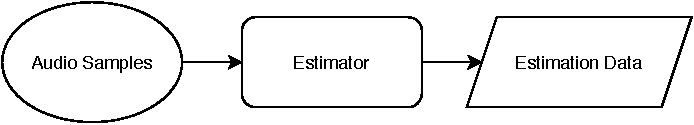
\includegraphics[width=\textwidth]{figures/approach/figEstimator.pdf}
    \end{center}
    \caption[Estimator Module]{Estimator Module}
    \label{fig:estimator}
\end{figure}


The evaluation of a system is highly coupled to the estimator.
Therefore it is up to the estimator to provide a suitable evaluation.
A well established error measure for vectors in general is the euclidean distance of two vectors
\begin{equation}
    \lVert \mathbf{\widetilde{x} - \mathbf{x}} \rVert_2 = \sqrt{(\tilde{x_1}-x_1)^2 + (\tilde{x_2}-x_2)^2 + ... + (\tilde{x_n}-x_n)^2}
\end{equation}
where
\begin{conditions}
    \mathbf{\widetilde{x}} & Estimation vector with length $n$ \\
    \mathbf{x} & True value vector with length $n$ \\
\end{conditions}
In the Evaluator Model the estimated values would be represented by $\mathbf{\widetilde{x}}$ and the real properties of the 3D data vectors by $\mathbf{x}$.
This approach will be used for the LOS localization estimator example in \chapref{chap:experiments}.
For non-vector types other approaches should be defined.

\begin{figure}[H]
    \begin{center}
    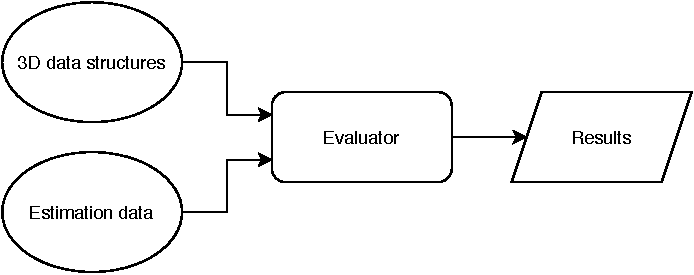
\includegraphics[width=\textwidth]{figures/approach/figEvaluator.pdf}
    \end{center}
    \caption[Evaluator Module]{Evaluator Module}
    \label{fig:evaluator}
\end{figure}

